\subsection{Четная функция}

Рассмотрим четную периодическую функцию с периодом $T = 2\pi$:

\begin{equation}
    f_2(t) = \sin\left(\frac{5}{2} \cos(t)\right)
\end{equation}

График этой функции приведен на рис.~\ref{fig:func_2}.

\begin{figure}[ht!]
    \centering
    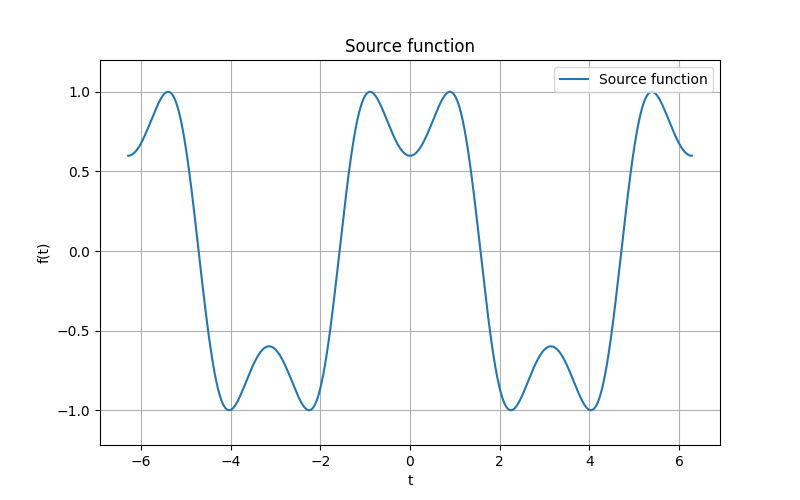
\includegraphics[width=\textwidth]{media/plots/func_2.png}
    \caption{График функции $f_2(t)$}
    \label{fig:func_2}
\end{figure}

\subsubsection{Вычисление коэффициентов Фурье}
Найдем коэффициенты ряда Фурье для этой функции:

\begin{equation}
    a_n = \frac{1}{\pi}\int\limits_{-\pi}^{\pi} \sin\left(\frac{5}{2} \cos\left(t\right)\right)\cos\left( n t \right) dt 
\end{equation}

\begin{equation}
    b_n = \frac{1}{\pi}\int\limits_{-\pi}^{\pi} \sin\left(\frac{5}{2} \cos\left(t\right)\right)\sin\left( n t \right) dt 
\end{equation}

\begin{equation}
    c_n = \frac{1}{2\pi}\int\limits_{-\pi}^{\pi}  \sin\left(\frac{5}{2} \cos\left(t\right)\right) e^{-int} dt 
\end{equation}

Уууупс, неберущийся интеграл... Ну а кому его брать то надо? Мне не надо, я поплакался в чате :)

\subsubsection{Вычисление коэффициентов Фурье с помощью программы}

\begin{lstlisting}[style=python_white, caption=Вычисление коэффициентов Фурье, label=lst:func_2]
func = np.vectorize(lambda x: np.sin(5/2 * np.cos(x)))
a, b = fourier(func, -np.pi, 2*np.pi, 3)
print_fourier_coefficients(a, b)
c = fourier_exp(func, -np.pi, 2*np.pi, 3)
print_fourier_exp_coefficients(c)
\end{lstlisting}

В результате выполнения программы (\ref{lst:func_2}) получим следующие значения (см. таблицу~\ref{tab:func_2}~и~\ref{tab:func_2_exp})~.

% table with coefficients
\begin{table}[h!]
    \centering
    \begin{tabular}{|c|c|c|}
        \hline
        $n$ & $a_n$ & $b_n$ \\
        \hline
        0 & 0.00012 & 0.0\\
        1 & 0.99431 & 0.0\\
        2 & 0.00012 & 0.0\\
        3 & -0.43308 & 0.0\\
        \hline
    \end{tabular}
    \caption{Коэффициенты Фурье для функции $f_2(t)$}
    \label{tab:func_2}
\end{table}

\begin{table}[h!]
    \centering
    \begin{tabular}{|c|c|}
        \hline
        $n$ & $c_n$ \\
        \hline
        -3 & -0.21654 \\
        -2 & -0.00006 \\
        -1 & 0.49715 \\
        0 & 0.00006 \\
        1 & 0.49715 \\
        2 & 0.00006 \\
        3 & -0.21654 \\
        \hline
    \end{tabular}
    \caption{Коэффициенты Фурье для функции $f_2(t)$ (комплексный случай)}
    \label{tab:func_2_exp}
\end{table}

\subsubsection{Построение графиков частичных сумм ряда Фурье}
В качество значений $N$ выберем $N = 1, 2, 3, 4, 5$. Для каждого значения $N$ вычислим частичную сумму ряда Фурье и построим график (см. рис.~\ref{fig:func_2_plot}~и~\ref{fig:func_2_plot_exp}).

\begin{lstlisting}[style=python_white, caption=Построение графиков частичных сумм ряда Фурье, label=lst:func_1_plot]
func = np.vectorize(lambda x: np.sin(5/2 * np.cos(x)))
calc_and_plot(func, -np.pi, 2 * np.pi, [1, 2, 3, 4, 5], './media/plots/func_2')
calc_and_plot_exp(func, -np.pi, 2 * np.pi, [1, 2, 3, 4, 5], './media/plots/func_2_exp')
\end{lstlisting}

% plot with partial sums
\begin{figure}[ht!]
    \centering
    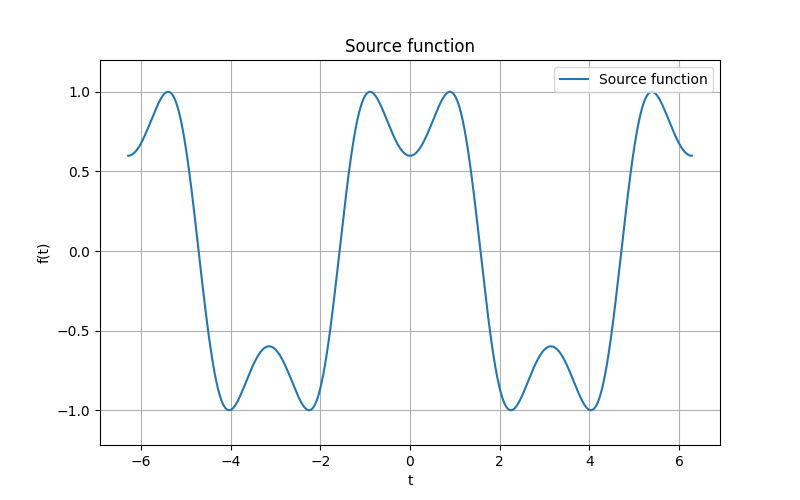
\includegraphics[width=0.49\textwidth]{media/plots/func_2.png}
    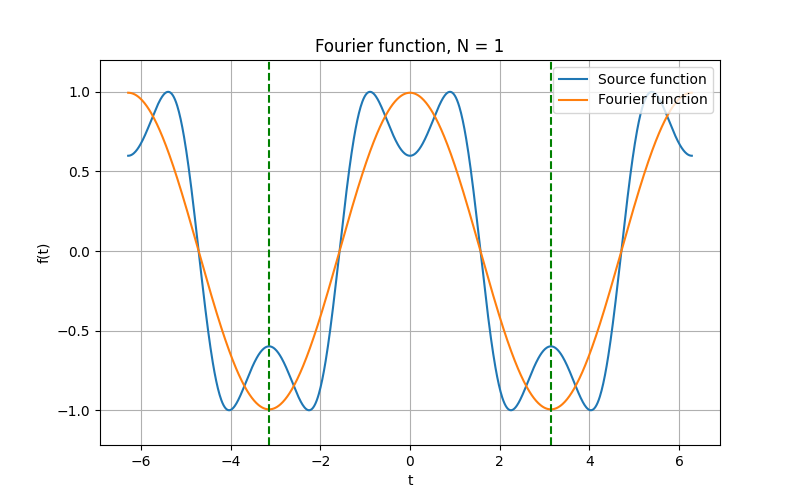
\includegraphics[width=0.49\textwidth]{media/plots/func_2_N_1.png}
    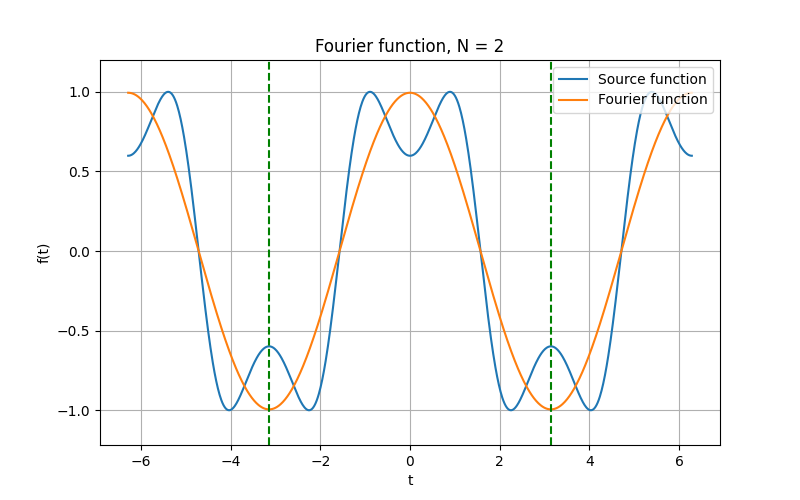
\includegraphics[width=0.49\textwidth]{media/plots/func_2_N_2.png}
    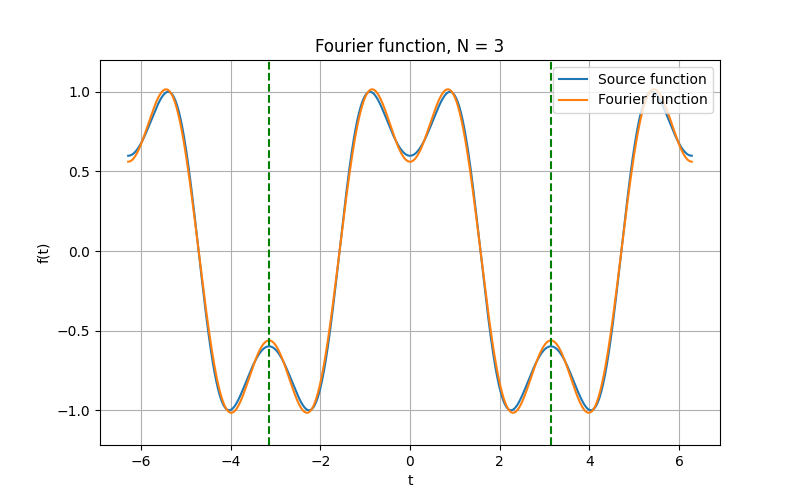
\includegraphics[width=0.49\textwidth]{media/plots/func_2_N_3.png}
    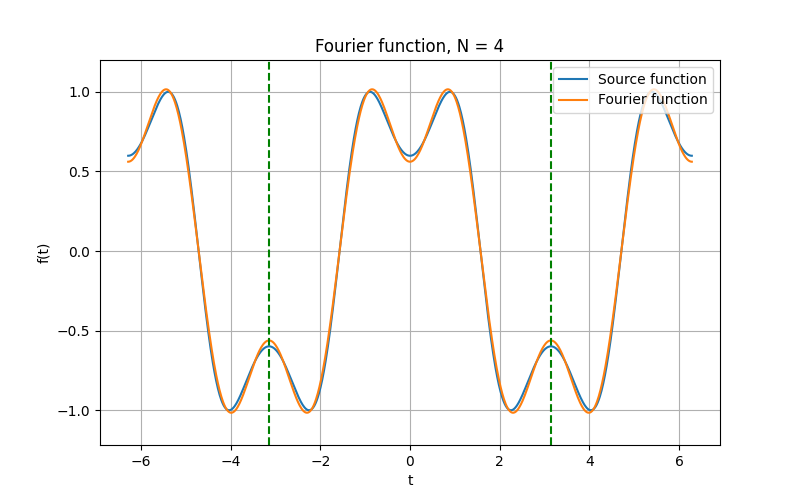
\includegraphics[width=0.49\textwidth]{media/plots/func_2_N_4.png}
    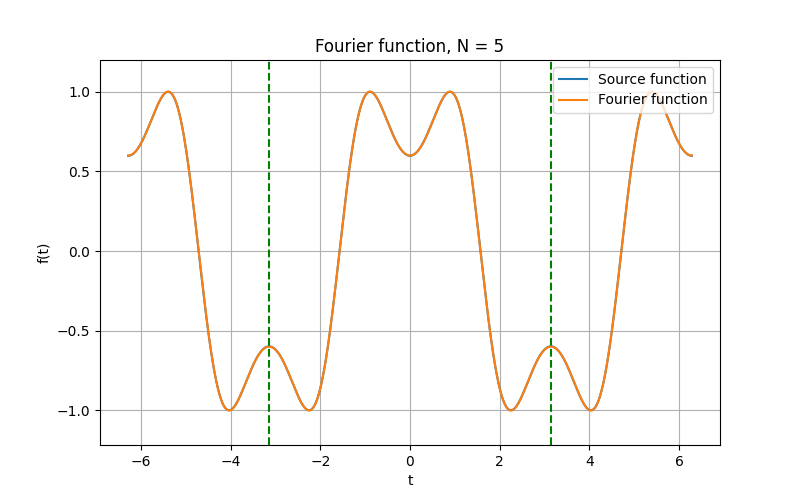
\includegraphics[width=0.49\textwidth]{media/plots/func_2_N_5.png}
    \caption{График частичных сумм ряда Фурье для функции $f_2(t)$}
    \label{fig:func_2_plot}
\end{figure}

\begin{figure}[ht!]
    \centering
    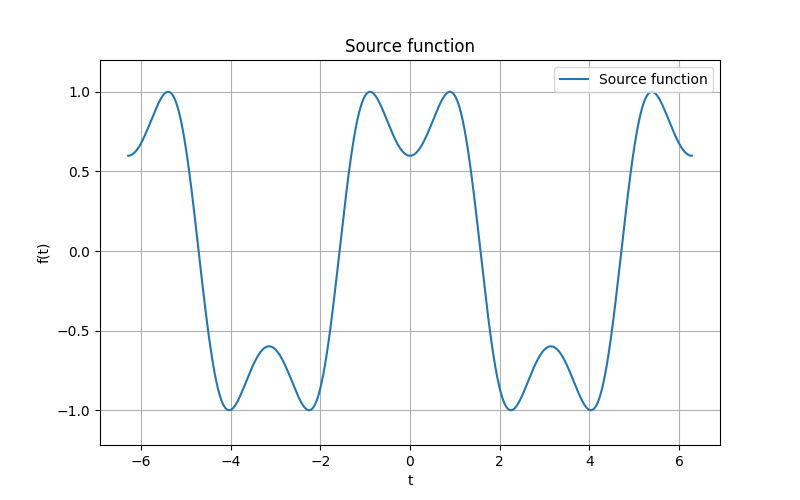
\includegraphics[width=0.49\textwidth]{media/plots/func_2_exp.png}
    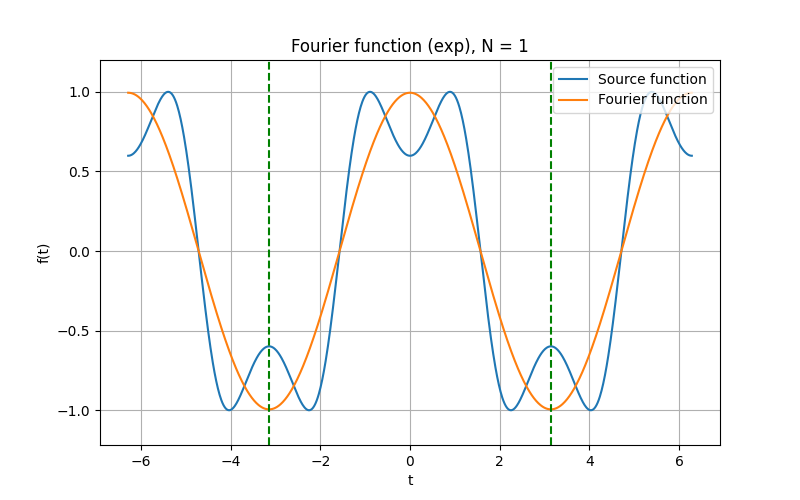
\includegraphics[width=0.49\textwidth]{media/plots/func_2_exp_N_1.png}
    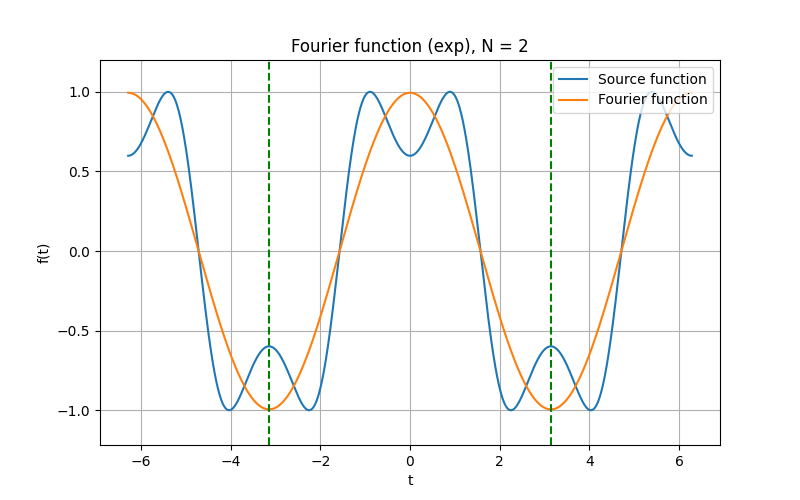
\includegraphics[width=0.49\textwidth]{media/plots/func_2_exp_N_2.png}
    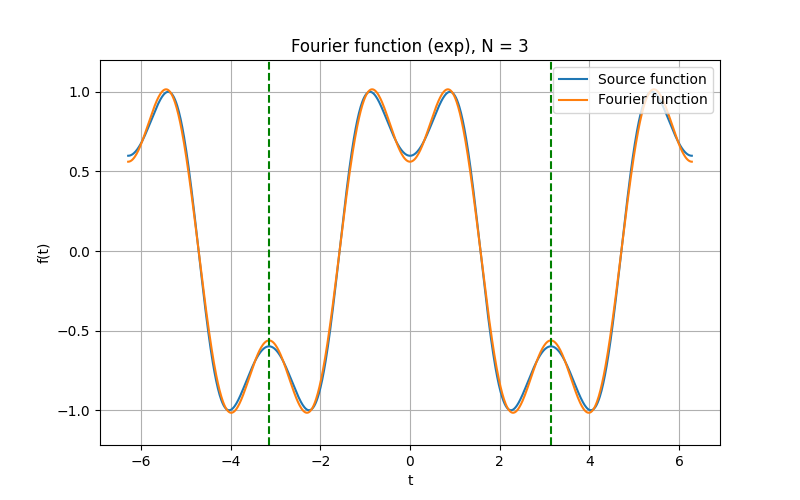
\includegraphics[width=0.49\textwidth]{media/plots/func_2_exp_N_3.png}
    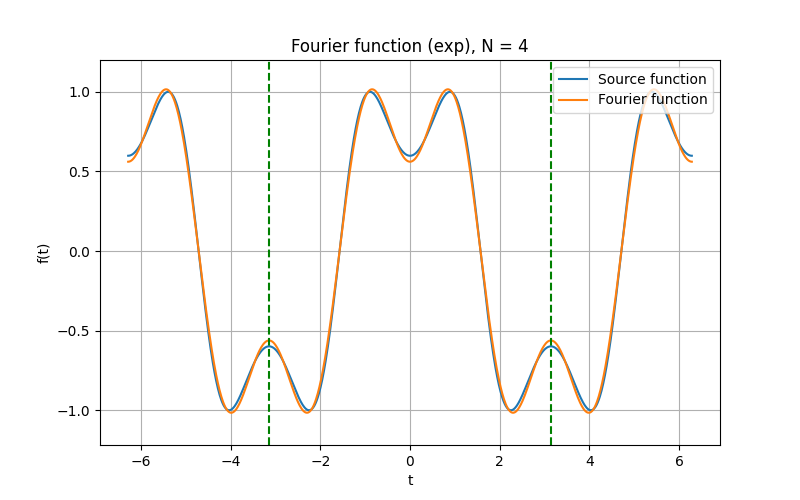
\includegraphics[width=0.49\textwidth]{media/plots/func_2_exp_N_4.png}
    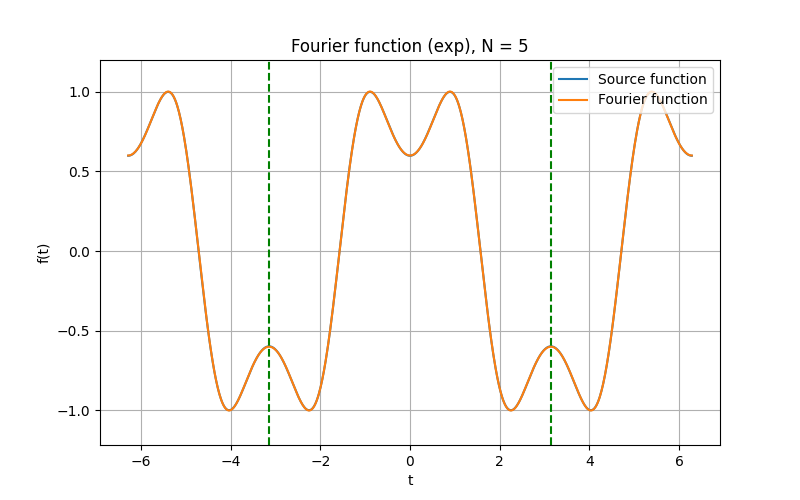
\includegraphics[width=0.49\textwidth]{media/plots/func_2_exp_N_5.png}
    \caption{График частичных сумм ряда Фурье для функции $f_2(t)$ (комплексный случай)}
    \label{fig:func_2_plot_exp}
\end{figure}

Видим, что при увеличении $N$ график частичной суммы ряда Фурье приближается к исходной функции. При $N = 5$ график частичной суммы ряда Фурье уже неотличим от исходной функции.

\FloatBarrier
\subsubsection{Проверка равенства Парсеваля}

Проверим равенство Парсеваля для функции $f_2(t)$:

Для этого воспользуемся функцией \texttt{perseval\_check} (см. листинг~\ref{lst:perseval_check}).
Мною была рассмотрена сумма трехсот коэффициентов. Этого оказалось достаточно для равенства квадрата нормы и суммы до 4 знака. 

\begin{table}[ht!]
    \centering
    \begin{tabular}{|c|c|c|}
        \hline
        $||f_2||^2$ & $2\pi \sum\limits_{n = -\infty}^{300} |c_n|^2$ & $\pi \left(\frac{a_0^2}{2} + \sum\limits_{n = 1}^{300} (a_n^2 + b_n^2)\right)$\\
        \hline
        3.69975 & 3.69999 & 3.69999 \\
        \hline
    \end{tabular}
    \caption{Проверка равенства Персеваля для функции $f_2(t)$}
    \label{tab:func_2_pers}
\end{table}
